\section{Hardware}

To achieve reliable real-time perception and efficient data handling, the system relies on a centralized hardware topology. A High-Performance Computing (HPC) unit acts as the main controller, interfacing directly with various external sensors and display modules. Figure \ref{fig:hw_arch} illustrates the physical connections between these components, highlighting the flow from data acquisition to user visualization. The key hardware elements include:

\begin{figure}[h]
    \centering
    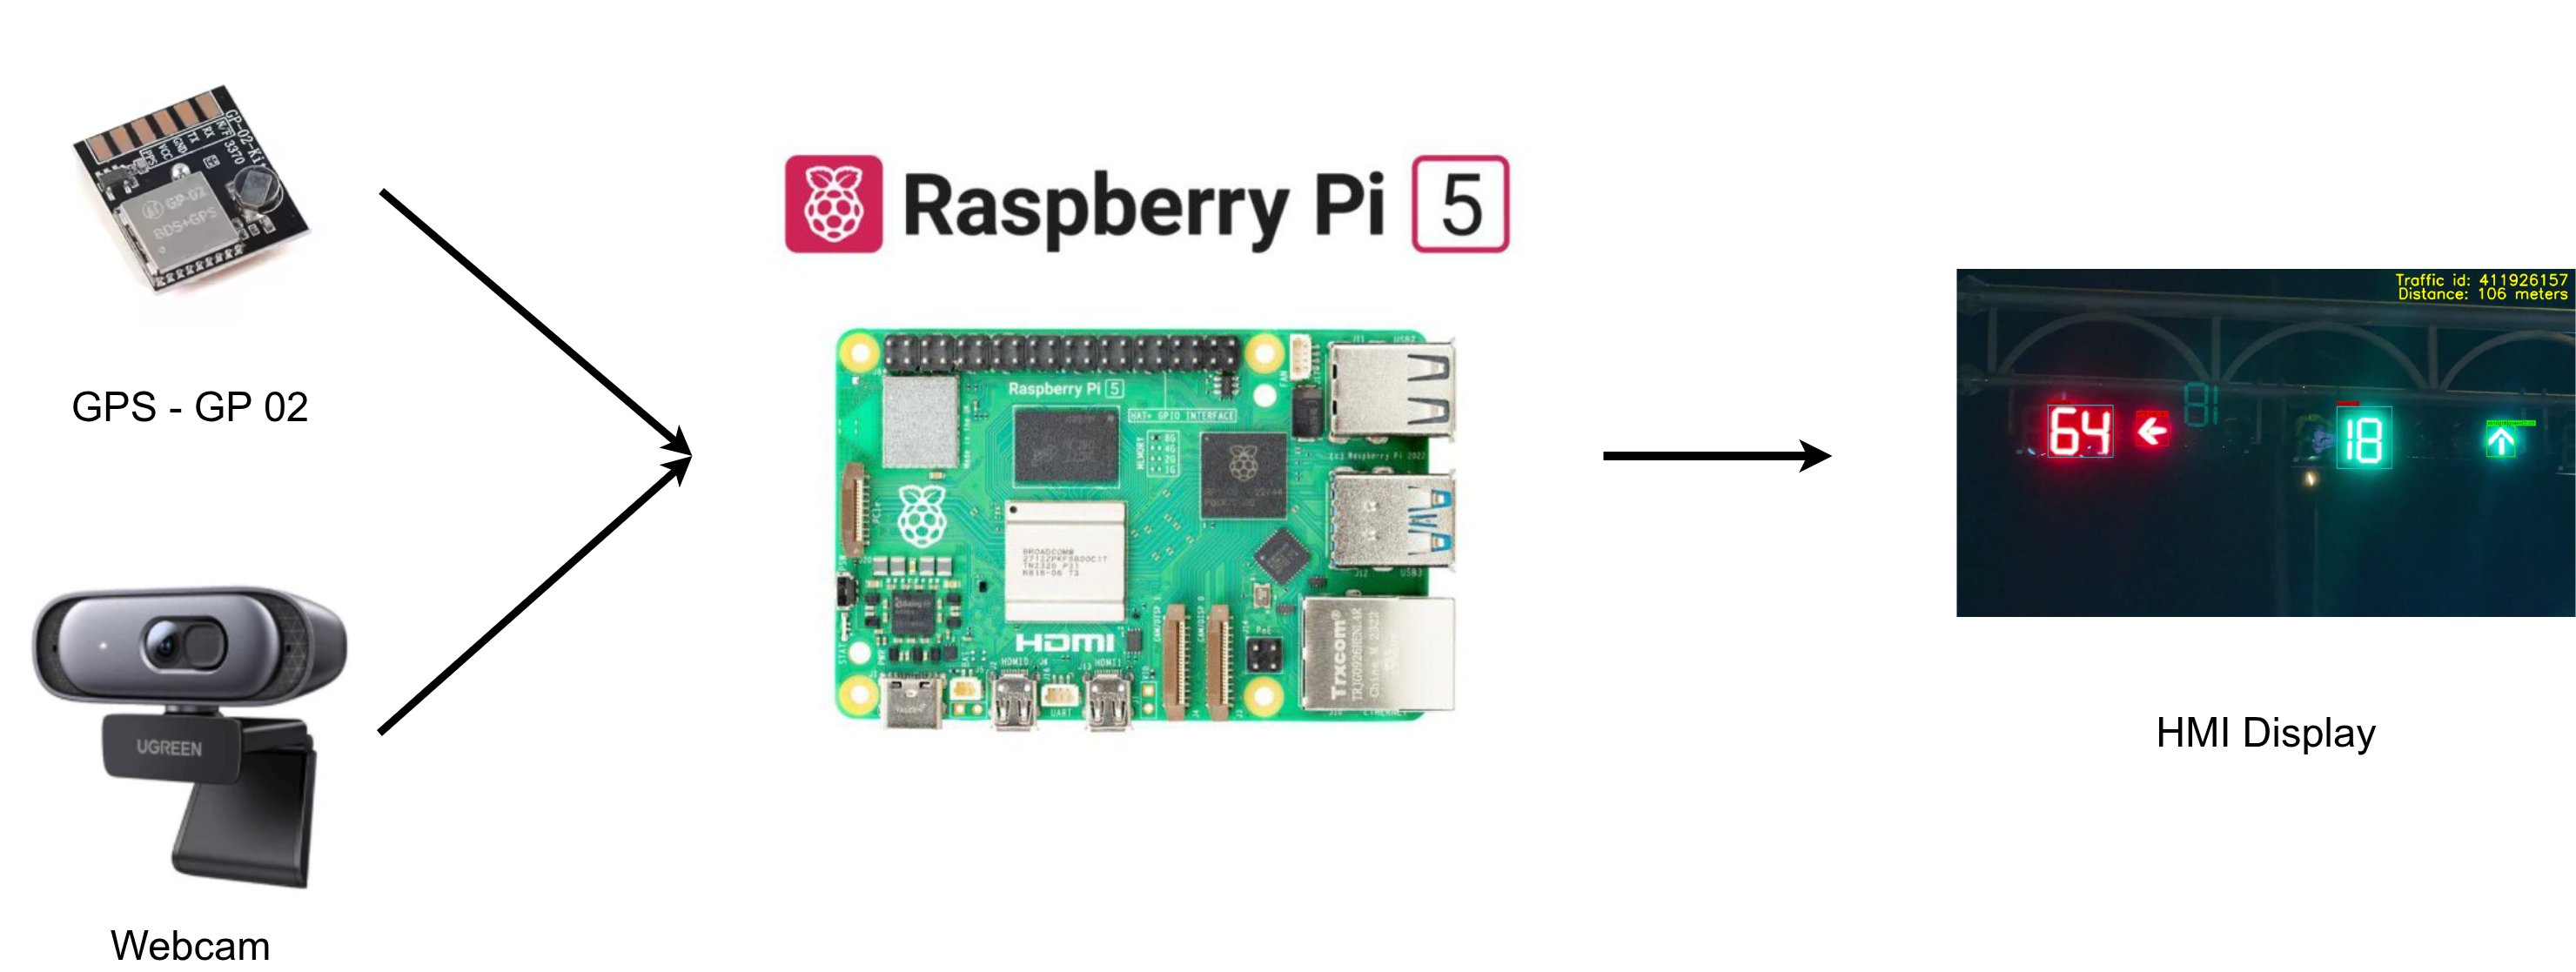
\includegraphics[width=0.8\textwidth]{Images/chapter2/hardware.png}
    \vspace{0.5cm}
    \caption{Hardware Architecture}
    \label{fig:hw_arch}
\end{figure}

\begin{itemize}
    \item \textbf{Raspberry Pi 5:} Acts as the central High-Performance Computing (HPC) unit, leveraging the Broadcom BCM2712 quad-core Arm Cortex-A76 processor clocked at 2.4GHz. This architecture delivers a \textbf{2-3x} performance boost over previous generations, providing the necessary computational overhead to execute complex Adaptive AUTOSAR applications, manage high-frequency DDS data distribution, and perform real-time edge-AI inference directly on the CPU.
    \item \textbf{USB Webcam:} Captures real-time video streams of the vehicle's surrounding environment, providing continuous visual input for the system's perception and object detection algorithms.
    \item \textbf{Ai-Thinker GP-02 GPS Module:} Acquires precise real-time geolocation data, including coordinates and velocity, which is essential for vehicle tracking and spatial awareness functions.
    \item \textbf{HMI Display:} Serves as the primary Human-Machine Interface, visually presenting critical information such as the real-time camera feed, object detection results, tracking data, and overall system status to the user.
\end{itemize}

